% !TeX root=../../doc.tex
\subsection{Landschaft}

Den wichtigsten „Drehort“, der für das Projekt benutzt wird, stellt das Informatikum der Universität Hamburg dar. Um für dieses zunächst möglichst genaue Umrisse zu ermitteln, übernahmen wir einen Kartenausschnitt aus \OSM. Dieser ist in \autoref{fig:ikum1} dargestellt, um 24,5° gegen den Uhrzeigersinn gedreht.

\begin{figure}[h]
	\centering
	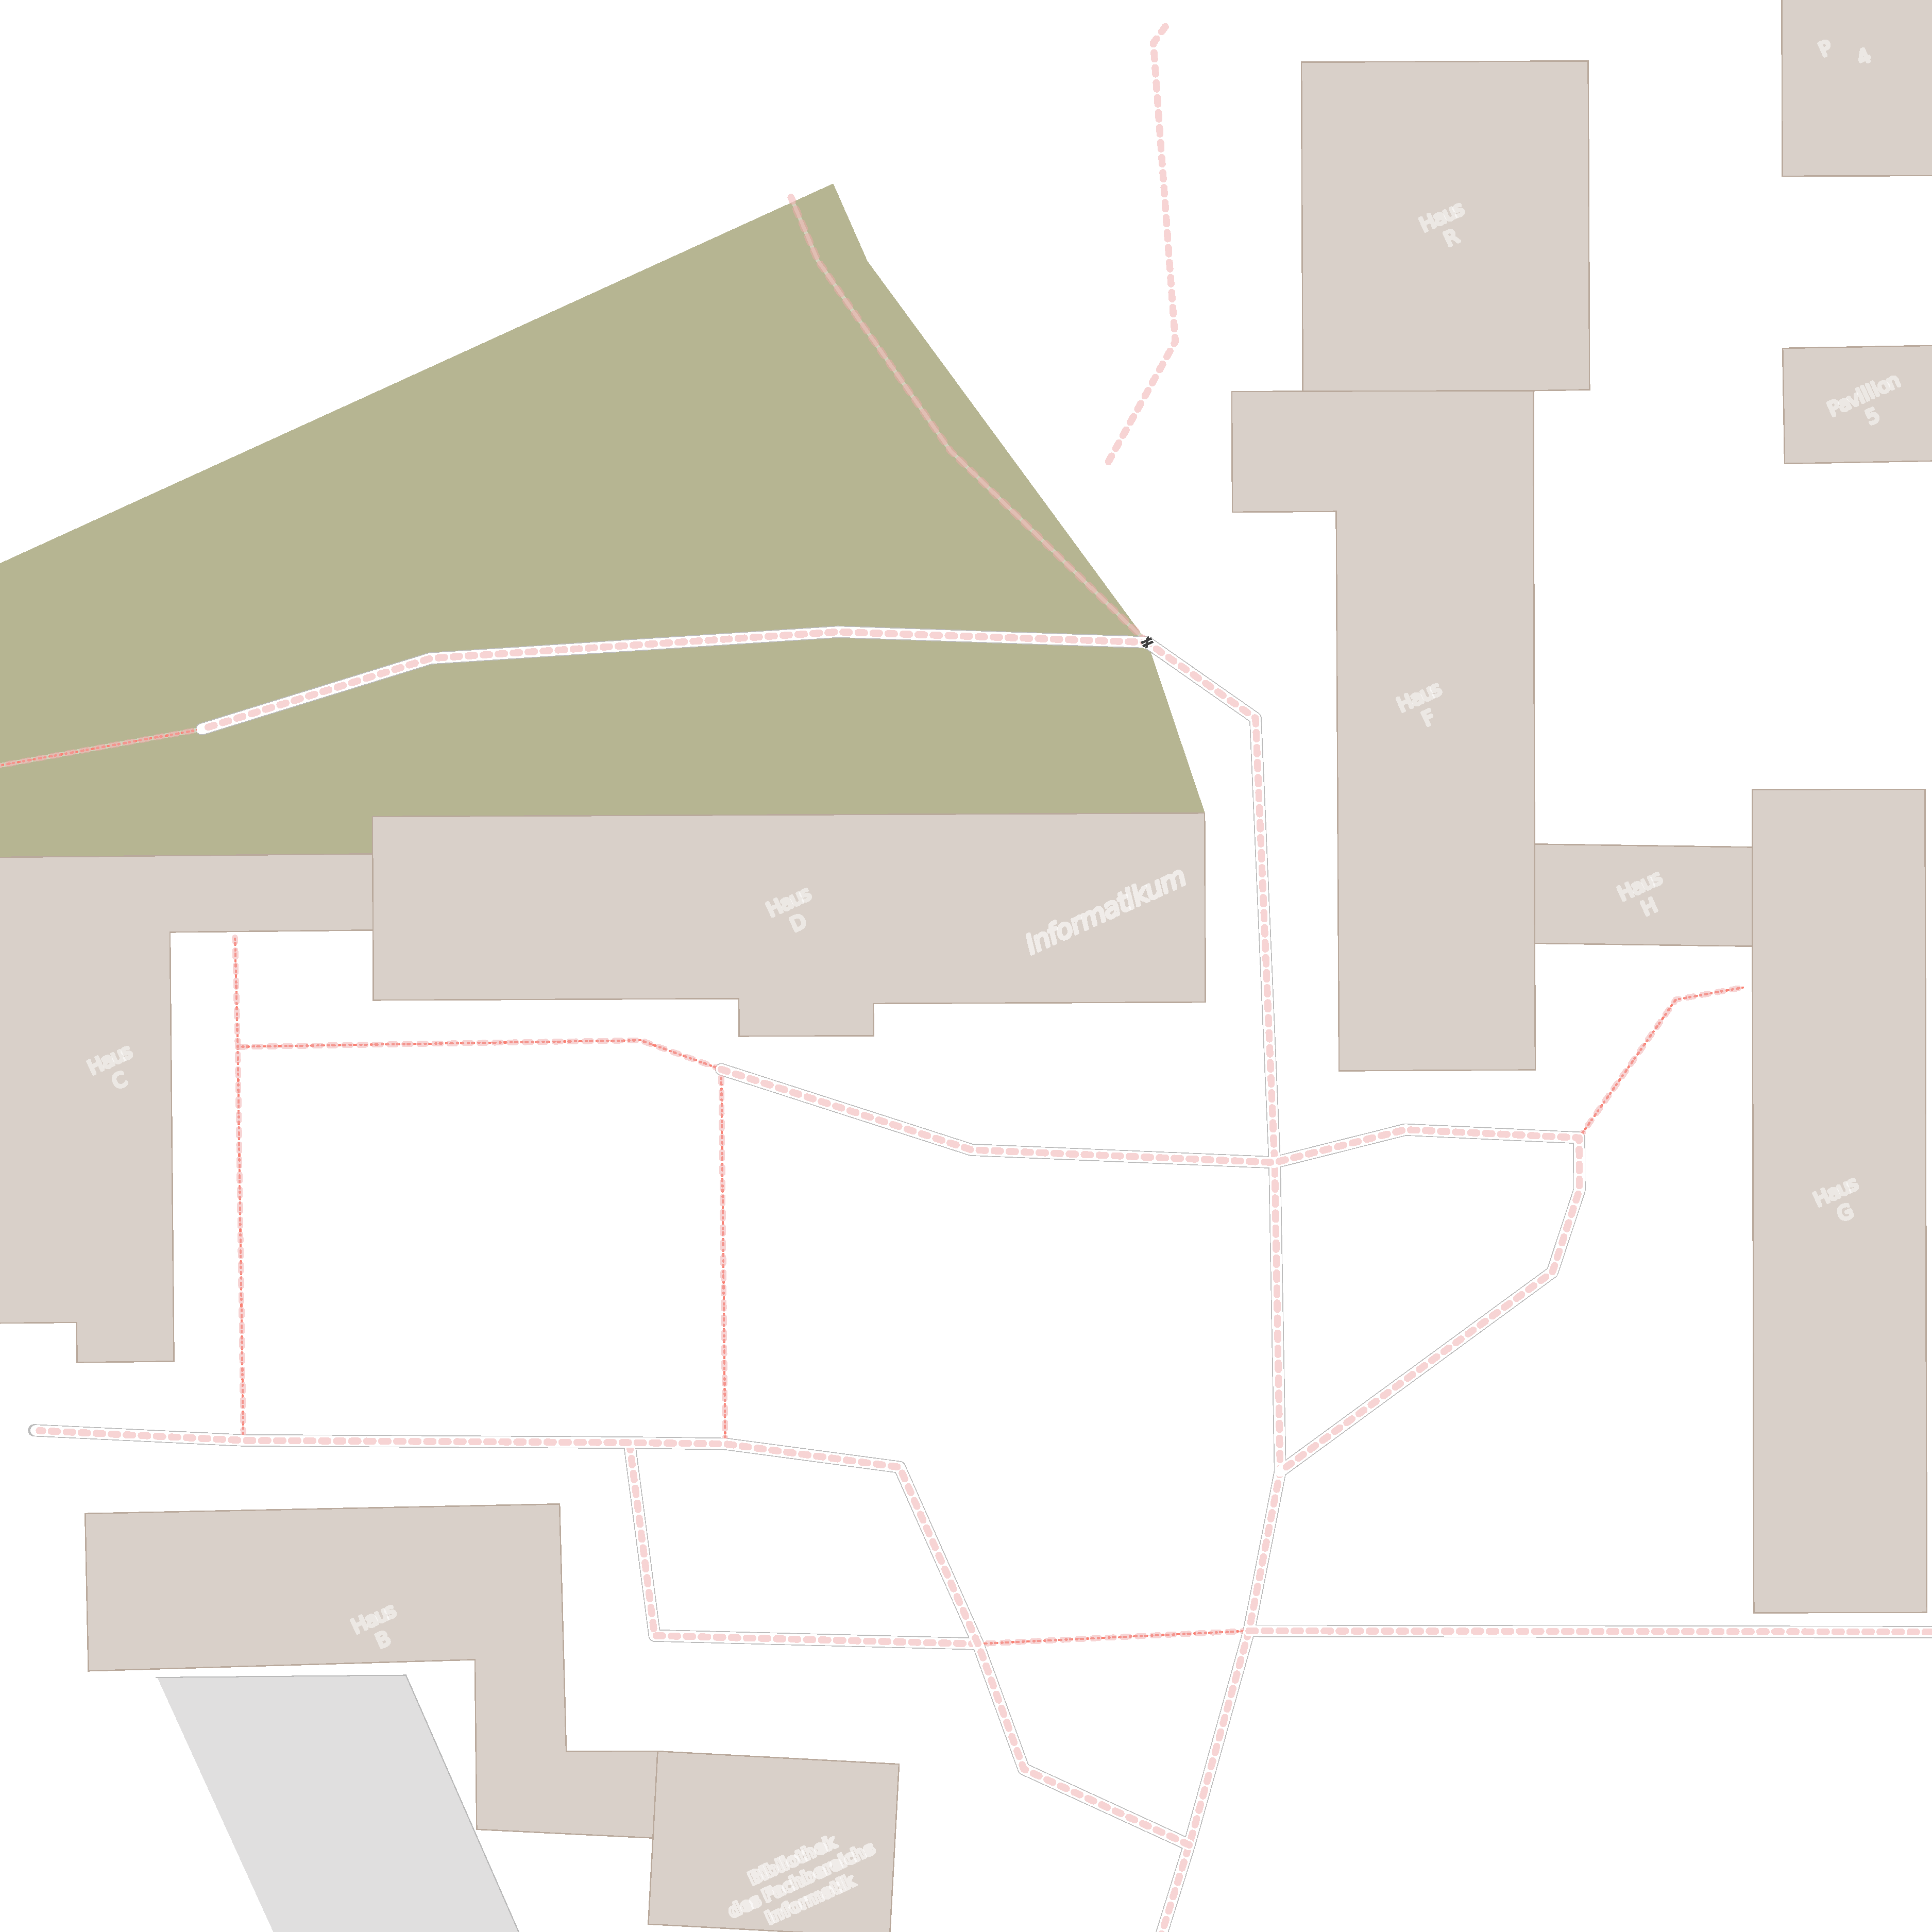
\includegraphics[width=0.55\linewidth]{Landscape/Informatikum/Informatikum1}
	\caption{Karte des Informatikums aus \OSM.}
	\label{fig:ikum1}
\end{figure}

Man sieht bereits, dass das Informatikum gut mithilfe von rechteckigen Formen dargestellt werden kann. Wir fertigten daher einen ersten Entwurf des Informatikums in \Illustrator an, wie er in \autoref{fig:ikum2} zu sehen ist. Dabei wurden die Koordinaten so normalisiert, dass ein Pixel des Modells einem Dezimeter der Wirklichkeit entspricht. Darüber hinaus sind die Werte gerundet, um ausschließlich rechteckige Formen benutzen zu können.

\begin{figure}[h]
	\centering
	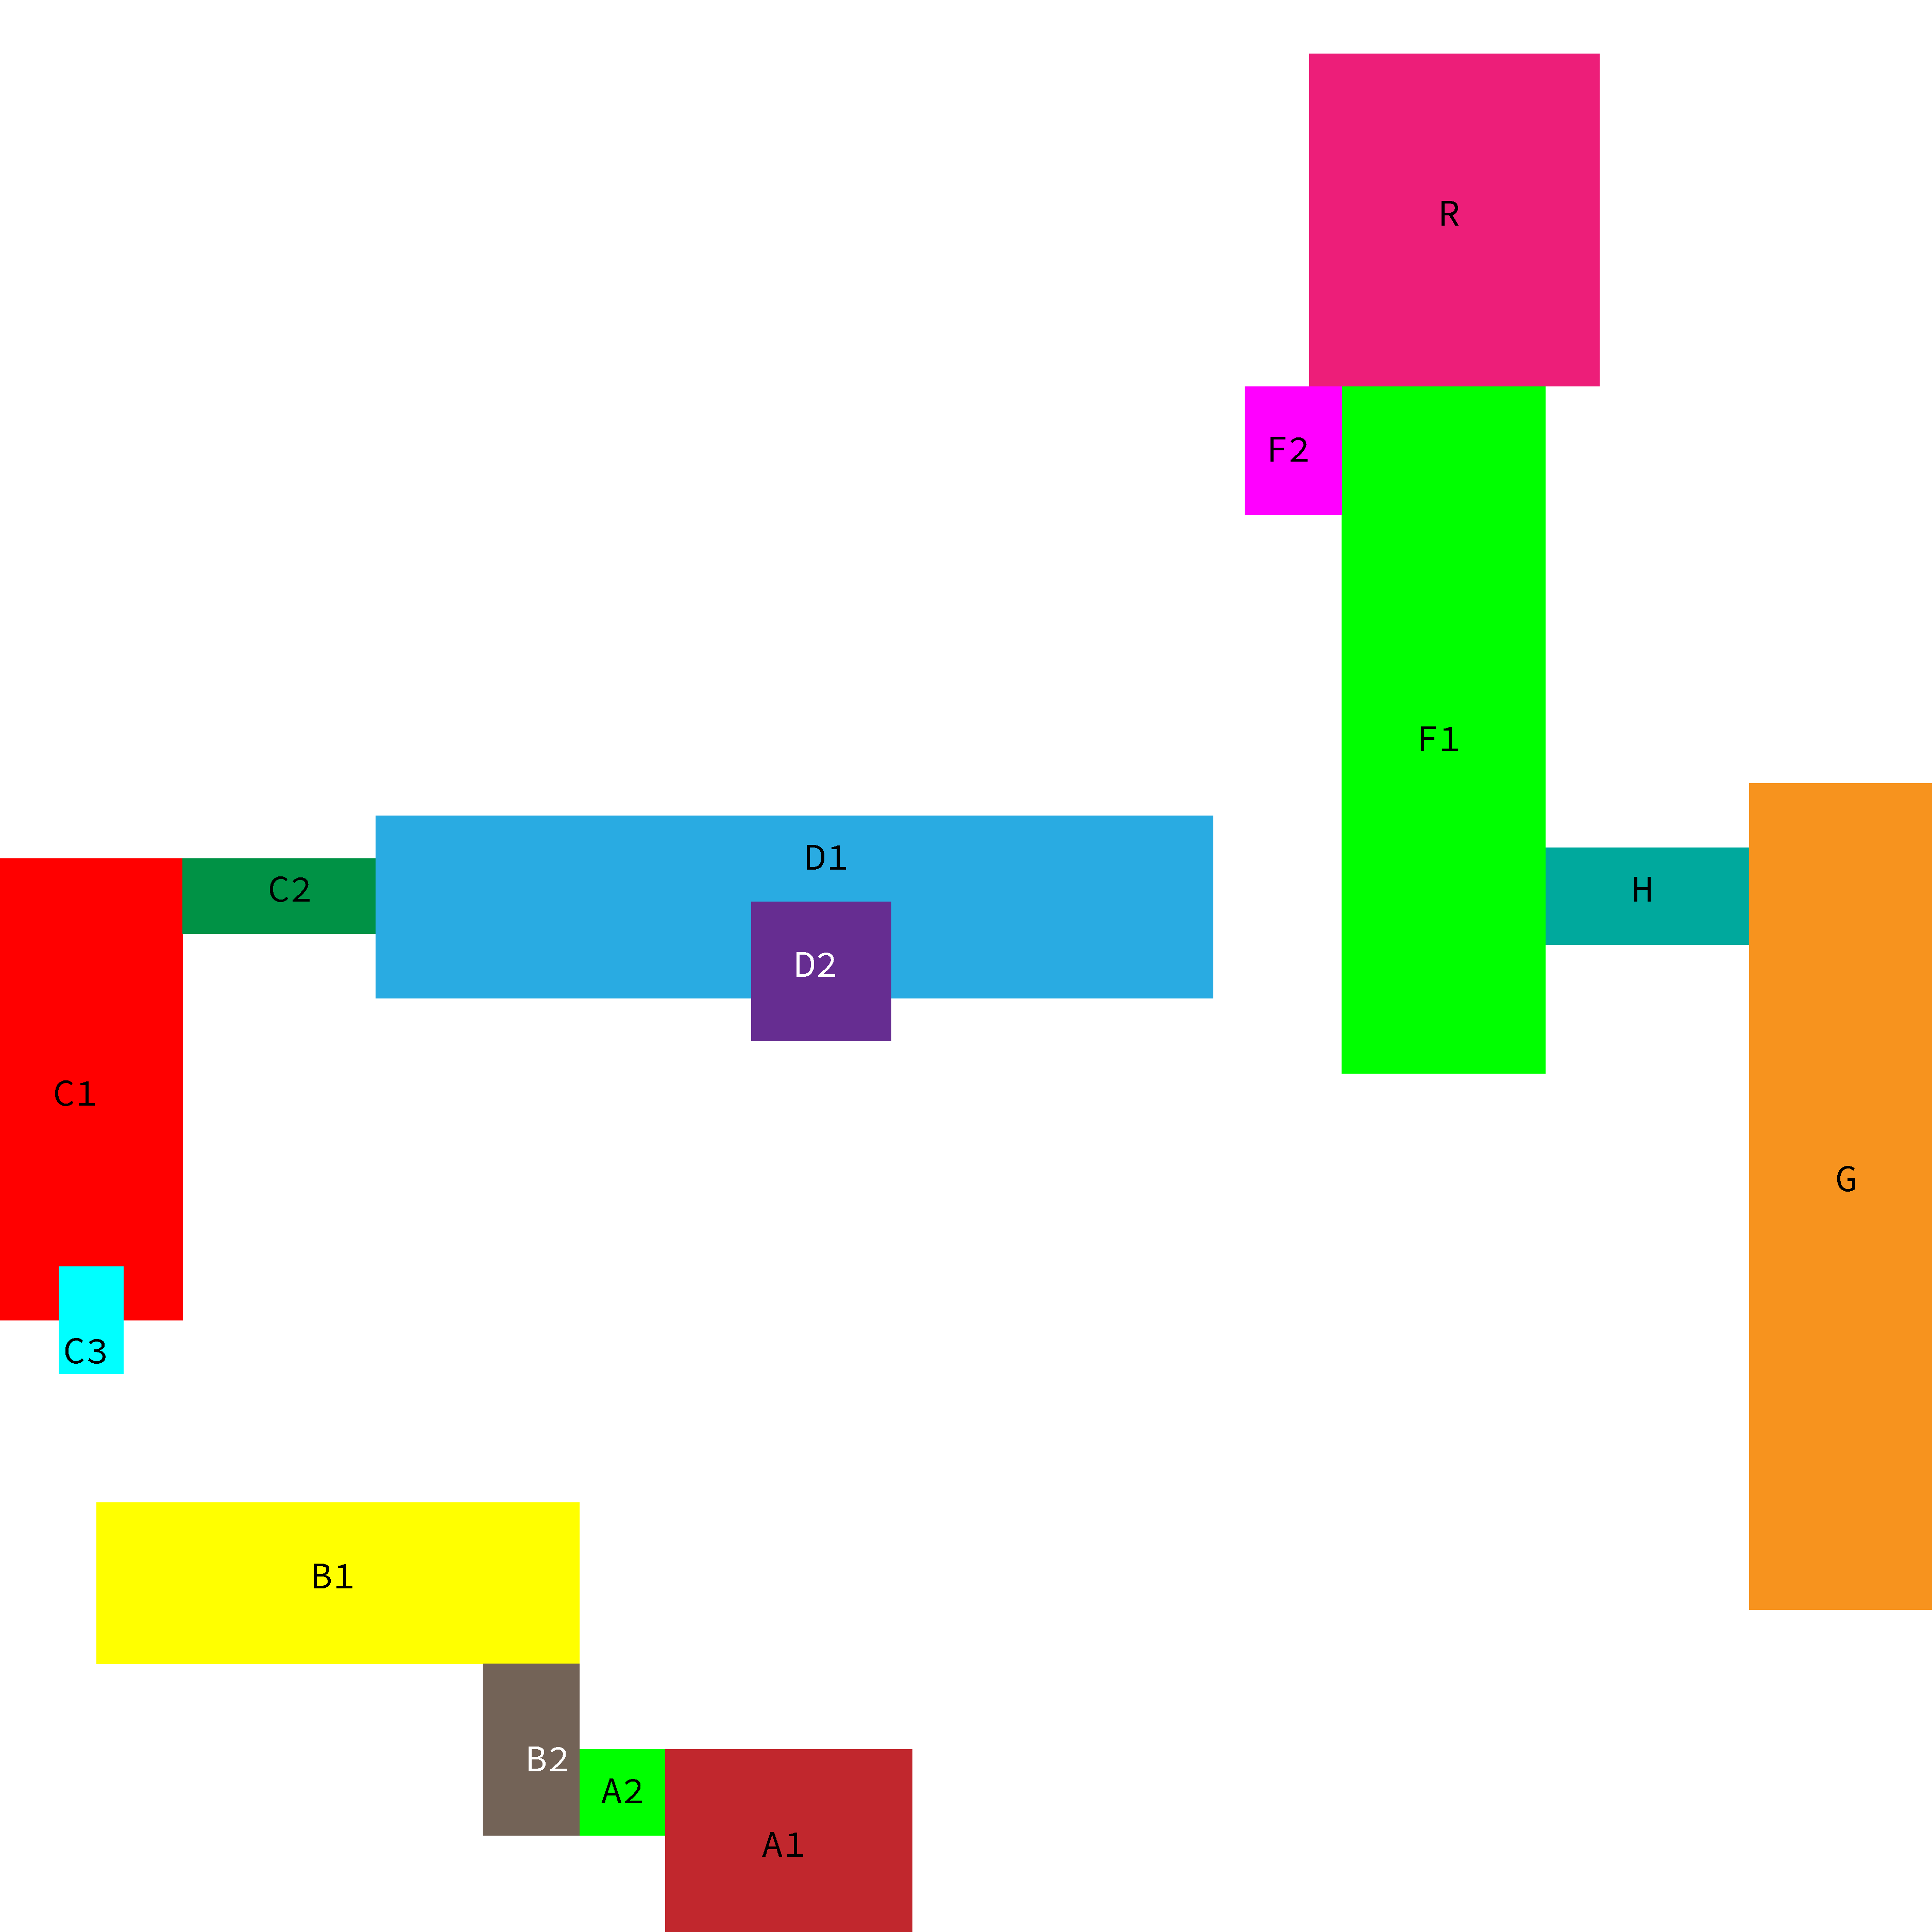
\includegraphics[width=0.55\linewidth]{Landscape/Informatikum/Informatikum2}
	\caption{Abstrahiertes Modell des Informatikums, erstellt mit \Illustrator.}
	\label{fig:ikum2}
\end{figure}

Nun wurden diese Formen und Koordinaten in \Povray eingepflegt. Über einfache Textverarbeitung können die Werte aus SVG-Dateien extrahiert und in \Povray"=Deklarationen umgewandelt werden. Mithilfe des Makros \texttt{Haus} wurde die Darstellung gerendert, die in \autoref{fig:ikum3} dargestellt ist.

\begin{figure}[h]
	\centering
	\includegraphics[width=0.55\linewidth]{Landscape/Informatikum/Informatikum3}
	\caption{Implementierung des ersten Modells mit \Povray.}
	\label{fig:ikum3}
\end{figure}